\section{Displacement correlations}\label{sec:5.6}

A dark-matter particle that transfers \SI{50}{keV} of momentum to a silicon nucleus in a cold crystal pushes on a particle that is spread over \SI{0.05}{\angstrom} by its zero-point motion. The phase $\vect{q}\cdot\vect{u}$ that the push imprints then varies by more than a radian across the nuclear wavefunction, and the expansion of $\ee^{\ii\vect{q}\cdot\vect{u}}$ to first order, which gave the single-phonon amplitude of \cref{sec:5.3}, no longer holds. In some events the nucleus takes up the momentum and the crystal is left in its ground state. Otherwise it emits one phonon, or two, or more, and at large enough momentum transfer the many-phonon sum turns into the free recoil of a lone nucleus. To find out how often each happens, we need the thermal averages of exponentials of displacements, at one time and at two. For a harmonic crystal both are exponentials of quadratic forms in $\vect{q}$, the Debye--Waller exponent $2W_\kappa(\vect{q})$ and the displacement correlation $\mathcal{C}_{\kappa\kappa'}(t)$, and both follow from the tensor $B_\kappa$ and the phonon modes of \cref{sec:5.3}. The same algebra describes the optical spectrum of a localized electron whose transition moves the nuclei around it, where it leads to the Franck--Condon factors and the Huang--Rhys factor.

\subsection{The Bloch identity}

The operator through which a momentum transfer $\vect{q}$ acts on the nucleus $\kappa$ in cell $\vect{R}$ is $\ee^{\ii\vect{q}\cdot\vect{X}}$, with $\vect{X} = \vect{R} + \vect{\tau}_\kappa + \vect{u}_{\vect{R}\kappa}$ (\cref{eq:5.1-X}). The lattice position contributes a phase, and the displacement contributes the operator $\ee^{\ii\vect{q}\cdot\vect{u}_{\vect{R}\kappa}}$. By \cref{eq:5.3-u}, $\vect{q}\cdot\vect{u}_{\vect{R}\kappa}$ is a linear combination of the phonon operators $b_{\vect{Q}\nu}$ and $b^\dagger_{\vect{Q}\nu}$. Its exponential contains every power of them and connects the thermal state to states with any number of extra phonons. The first question is its average.

For a classical Gaussian variable $x$ with zero mean, the average of $\ee^{\ii qx}$ is $\ee^{-q^2\langle x^2\rangle/2}$ (\cref{eq:C.6-generating}). A harmonic crystal in thermal equilibrium makes the same statement for operators. Its density matrix $\ee^{-\beta H_{\mathrm{N}}}/\mathcal{Z}$ is Gaussian in the normal coordinates and momenta, because $H_{\mathrm{N}}$ of \cref{eq:5.3-Hb} is quadratic in them. For any operator $\op{A}$ linear in the phonon operators,
\begin{equation*}
  \langle\ee^{\op{A}}\rangle = \ee^{\langle\op{A}^2\rangle/2} ,
\end{equation*}
which is Bloch's identity, \cref{eq:C.6-bloch}. Expanded in powers of $\op{A}$, it is Wick's theorem: the average of $\op{A}^{2n}$ is the sum over the $(2n)!/(2^nn!)$ ways of pairing the $2n$ factors, each pair worth $\langle\op{A}^2\rangle$.

To prove it, take one oscillator, $H = \omega_0(d^\dagger d + \tfrac12)$ as in \cref{app:C.6}, in thermal equilibrium at temperature $T = 1/\beta$, with $n_{\mathrm{B}} = n_{\mathrm{B}}(\omega_0)$, and let $\op{A} = \eta_1d + \eta_2d^\dagger$ with arbitrary complex $\eta_1$ and $\eta_2$, so that $\op{A}$ need not be Hermitian. Consider $F(\theta) = \langle\ee^{\theta\op{A}}\rangle$ as a function of a real parameter $\theta$. The proof uses two facts. The commutators $[\op{A}, d] = -\eta_2$ and $[\op{A}, d^\dagger] = \eta_1$ are numbers. By \cref{eq:C.6-hadamard}, the transformation by $\ee^{\theta\op{A}}$ therefore only shifts the ladder operators,
\begin{equation*}
  d\,\ee^{\theta\op{A}} = \ee^{\theta\op{A}}\,(d + \theta\eta_2), \qquad d^\dagger\,\ee^{\theta\op{A}} = \ee^{\theta\op{A}}\,(d^\dagger - \theta\eta_1) .
\end{equation*}
The cyclic property of the trace, in turn, moves a ladder operator past the Boltzmann factor at a known cost, as in the proof of Wick's theorem in \cref{app:D.11}: $d\,\ee^{-\beta H} = \ee^{-\beta\omega_0}\ee^{-\beta H}d$, since removing a quantum lowers $H$ by $\omega_0$, and $d^\dagger\ee^{-\beta H} = \ee^{+\beta\omega_0}\ee^{-\beta H}d^\dagger$. As a result, $\langle\ee^{\theta\op{A}}d\rangle = \Tr[d\,\ee^{-\beta H}\ee^{\theta\op{A}}]/\mathcal{Z} = \ee^{-\beta\omega_0}\langle d\,\ee^{\theta\op{A}}\rangle$, and combined with the shift,
\begin{equation*}
  \langle d\,\ee^{\theta\op{A}}\rangle = \ee^{-\beta\omega_0}\langle d\,\ee^{\theta\op{A}}\rangle + \theta\eta_2F(\theta), \qquad
  \langle d\,\ee^{\theta\op{A}}\rangle = \frac{\theta\eta_2F(\theta)}{1 - \ee^{-\beta\omega_0}} = \theta\eta_2\,(n_{\mathrm{B}} + 1)\,F(\theta) .
\end{equation*}
The same steps for $d^\dagger$ give $\langle d^\dagger\ee^{\theta\op{A}}\rangle = \ee^{\beta\omega_0}\langle d^\dagger\ee^{\theta\op{A}}\rangle - \theta\eta_1F(\theta)$, and $\langle d^\dagger\ee^{\theta\op{A}}\rangle = \theta\eta_1\,n_{\mathrm{B}}\,F(\theta)$. The derivative of $F$ is then
\begin{equation*}
  F'(\theta) = \eta_1\langle d\,\ee^{\theta\op{A}}\rangle + \eta_2\langle d^\dagger\ee^{\theta\op{A}}\rangle = \theta\,\eta_1\eta_2\,(2n_{\mathrm{B}} + 1)\,F(\theta) = \theta\,\langle\op{A}^2\rangle\,F(\theta) ,
\end{equation*}
since $\langle\op{A}^2\rangle = \eta_1\eta_2\langle dd^\dagger + d^\dagger d\rangle = \eta_1\eta_2(2n_{\mathrm{B}} + 1)$, the averages of $d^2$ and $d^{\dagger2}$ being zero. With $F(0) = 1$ the solution is $F(\theta) = \ee^{\theta^2\langle\op{A}^2\rangle/2}$, which at $\theta = 1$ is Bloch's identity. For several independent modes in thermal equilibrium, $\op{A} = \sum_\gamma\op{A}_\gamma$ is a sum of commuting pieces, one per mode, the exponential factorizes, and the average in the Gibbs state of \cref{sec:2.5} factorizes too. The exponents add, and $\sum_\gamma\langle\op{A}_\gamma^2\rangle = \langle\op{A}^2\rangle$, because the cross terms $\langle\op{A}_\gamma\op{A}_{\gamma'}\rangle = \langle\op{A}_\gamma\rangle\langle\op{A}_{\gamma'}\rangle$ vanish for $\gamma \ne \gamma'$. The identity therefore holds for any $\op{A}$ linear in the operators of a set of harmonic modes.

The hypotheses are the ones the proof used. The operator must be linear in $d$ and $d^\dagger$, so that its commutators are numbers, and the state must be the thermal state of a quadratic Hamiltonian, so that the trace moves each ladder operator at the cost of a number. In an anharmonic crystal neither holds exactly. The logarithm of $\langle\ee^{\op{A}}\rangle$ is then a series in the cumulants of $\op{A}$, of which the harmonic crystal has only the second. The anharmonic terms of \cref{sec:5.7} make the fourth cumulant nonzero, and the Debye--Waller exponent acquires a correction that grows with temperature faster than $T$.

With $\op{A} = \ii\vect{q}\cdot\vect{u}_{\vect{R}\kappa}$, $\langle\op{A}^2\rangle = -\langle(\vect{q}\cdot\vect{u}_{\vect{R}\kappa})^2\rangle = -\sum_{\alpha\beta}q^\alpha B^{\alpha\beta}_\kappa q^\beta$, with the displacement tensor $B_\kappa$ of \cref{eq:5.3-B}.
\begin{keyresult}[Debye--Waller factor]
For a nucleus $\kappa$ of a harmonic crystal in thermal equilibrium,
\begin{equation}
  \bigl\langle\ee^{\ii\vect{q}\cdot\vect{u}_{\vect{R}\kappa}}\bigr\rangle = \ee^{-W_\kappa(\vect{q})} , \qquad
  2W_\kappa(\vect{q}) = \vect{q}\cdot B_\kappa\cdot\vect{q} = \frac1N\sum_{\vect{Q}\nu}\frac{|\vect{q}\cdot\vect{e}_{\kappa\nu}(\vect{Q})|^2}{2M_\kappa\,\omega_{\vect{Q}\nu}}\,\coth\frac{\omega_{\vect{Q}\nu}}{2T} ,
  \label{eq:5.6-W}
\end{equation}
the same in every cell. At a site of cubic symmetry, $2W_\kappa(\vect{q}) = q^2\langle u_x^2\rangle$.
\end{keyresult}
The factor $\ee^{-W_\kappa}$ is an amplitude: the probability amplitude for the nucleus to absorb $\vect{q}$ and leave the lattice in the state it found it in, averaged over that state. The probability is its square, the \emph{Debye--Waller factor} $\ee^{-2W_\kappa(\vect{q})}$, and $W_\kappa(\vect{q})$ is the Debye--Waller exponent. In X-ray and neutron diffraction the factor multiplies the intensity of every Bragg peak, which is how $B_\kappa$ is measured; in silicon at \SI{293}{K}, with the reference value $\langle u_x^2\rangle = \SI{5.94e-3}{\angstrom^2}$ of \cref{we:5-u2}, it reduces the (111) reflection, at $|\vect{G}_{111}| = \sqrt3\,2\pi/a = \SI{3.95}{keV}$, by only \SI{2.4}{\percent}. Note that the electron--phonon literature also uses the name ``Debye--Waller'' for the term of second order in the displacements of the electron--phonon interaction. That term shifts electronic energies and is a different object, the Allen--Heine term of \cref{sec:6.3} (\cref{app:A.6}); in this book the name means \cref{eq:5.6-W} only.

\Cref{eq:5.6-W} inherits the structure of $B_\kappa$. The exponent grows as $q^2$, and it is largest along directions in which the nucleus is soft. Each mode contributes in proportion to the projection of $\vect{q}$ on its polarization, divided by its energy, and weighted by $2n_{\vect{Q}\nu} + 1$, which grows from one at $T = 0$ to $2T/\omega_{\vect{Q}\nu}$ at high temperature. For one species at a cubic site, $2W_\kappa = q^2\langle u^2\rangle/3$, and in the Debye model \cref{eq:5.3-debye} gives
\begin{equation}
  2W_\kappa(\vect{q}) = \frac{3q^2}{4M_\kappa\omega_{\mathrm{D}}}\Bigl[1 + 4\Bigl(\frac{T}{\omega_{\mathrm{D}}}\Bigr)^2\int_0^{\omega_{\mathrm{D}}/T}\frac{x\,\dd x}{\ee^x - 1}\Bigr] .
  \label{eq:D.15-debye}
\end{equation}
At $T = \omega_{\mathrm{D}}$ the bracket is $4.11$: the exponent is four times its zero-point value. At $T = 0$ it is
\begin{equation*}
  2W_\kappa(\vect{q}) = \frac{3q^2}{4M_\kappa\omega_{\mathrm{D}}} = \frac32\,\frac{E_R}{\omega_{\mathrm{D}}} , \qquad E_R = \frac{q^2}{2M_\kappa} ,
\end{equation*}
with $E_R$ the recoil energy that a free nucleus would take (\cref{sec:1.3}). This is the scale that controls everything below: the lattice stays in its ground state with high probability as long as the recoil energy is small compared with typical phonon energies, and almost never once it is large. For numbers we use the computed spectrum, since the Debye model misses the flat transverse acoustic branches (\cref{we:5-u2}).

\subsection{The displacement correlation}

A scattering rate needs more than an average. By \cref{eq:4.2-Sab}, the dynamic structure factor of the nuclei is the Fourier transform in time of the correlation of the density operator at time $t$ with its adjoint at time zero. For one nucleus the density is $\ee^{\ii\vect{q}\cdot\vect{X}}$, and the static phases cancel between the two factors, leaving
\begin{equation*}
  \bigl\langle\ee^{-\ii\vect{q}\cdot\vect{u}_{\vect{R}\kappa}(t)}\,\ee^{\ii\vect{q}\cdot\vect{u}_{\vect{R}\kappa}(0)}\bigr\rangle ,
\end{equation*}
with the Heisenberg operators $b_{\vect{Q}\nu}(t) = b_{\vect{Q}\nu}\ee^{-\ii\omega_{\vect{Q}\nu}t}$ of \cref{sec:5.3}. The two exponents are still linear in the phonon operators, but they do not commute, and Bloch's identity has to be combined with the Baker--Campbell--Hausdorff formula. For two operators $\op{A}$ and $\op{B}$ linear in the phonon operators, the commutator is a number, $\ee^{\op{A}}\ee^{\op{B}} = \ee^{\op{A} + \op{B}}\ee^{[\op{A}, \op{B}]/2}$ (\cref{eq:C.6-BCH}), and Bloch's identity applied to $\op{A} + \op{B}$ leads to
\begin{equation*}
  \langle\ee^{\op{A}}\ee^{\op{B}}\rangle = \exp\Bigl[\tfrac12\langle\op{A}^2\rangle + \tfrac12\langle\op{B}^2\rangle + \langle\op{A}\op{B}\rangle\Bigr] ,
\end{equation*}
\cref{eq:C.6-product}. With $\op{A} = -\ii\vect{q}\cdot\vect{u}_{\vect{R}\kappa}(t)$ and $\op{B} = \ii\vect{q}\cdot\vect{u}_{\vect{R}\kappa}(0)$, the first two terms are $-W_\kappa(\vect{q})$ each, since the thermal state is stationary and the average of a square does not depend on time. The third term is a correlation of two displacements at different times. Inserting \cref{eq:5.3-u} twice, the averages $\langle b_{\vect{Q}\nu}b^\dagger_{\vect{Q}\nu}\rangle = n_{\vect{Q}\nu} + 1$ and $\langle b^\dagger_{\vect{Q}\nu}b_{\vect{Q}\nu}\rangle = n_{\vect{Q}\nu}$ now come with the phases $\ee^{-\ii\omega_{\vect{Q}\nu}t}$ and $\ee^{+\ii\omega_{\vect{Q}\nu}t}$, and the \emph{displacement correlation} of the nuclei $\kappa$ and $\kappa'$ is
\begin{equation}
  \mathcal{C}^{\alpha\beta}_{\kappa\kappa'}(\vect{R},t) = \bigl\langle u^\alpha_{\vect{R}\kappa}(t)\,u^\beta_{\vect{0}\kappa'}(0)\bigr\rangle
  = \frac1N\sum_{\vect{Q}\nu}\frac{e^\alpha_{\kappa\nu}(\vect{Q})\,e^\beta_{\kappa'\nu}(\vect{Q})^*\,\ee^{\ii\vect{Q}\cdot\vect{R}}}{2\omega_{\vect{Q}\nu}\sqrt{M_\kappa M_{\kappa'}}}\Bigl[(n_{\vect{Q}\nu} + 1)\,\ee^{-\ii\omega_{\vect{Q}\nu}t} + n_{\vect{Q}\nu}\,\ee^{\ii\omega_{\vect{Q}\nu}t}\Bigr] ,
  \label{eq:5.6-C}
\end{equation}
For one nucleus, $\vect{R} = \vect{0}$ and $\kappa' = \kappa$, we write $\mathcal{C}_{\kappa\kappa}(t)$. Its value at $t = 0$ is the displacement tensor, $\mathcal{C}_{\kappa\kappa}(0) = B_\kappa$. The term with $n_{\vect{Q}\nu} + 1$ creates a phonon at time zero and removes it at time $t$, and oscillates at the positive frequency $\omega_{\vect{Q}\nu}$; the term with $n_{\vect{Q}\nu}$ absorbs a thermal phonon first, and it vanishes at $T = 0$. Unlike $B_\kappa$, the correlation is complex, because $\vect{u}(t)$ and $\vect{u}(0)$ do not commute. Its imaginary part, $\Imag\mathcal{C}_{\kappa\kappa}(t) = -\sum_{\vect{Q}\nu}\vect{e}_{\kappa\nu}\vect{e}^*_{\kappa\nu}\sin(\omega_{\vect{Q}\nu}t)/(2NM_\kappa\omega_{\vect{Q}\nu})$, does not depend on temperature; we will see that it carries the recoil energy.
\begin{keyresult}[Generating formula]
For a nucleus $\kappa$ of a harmonic crystal in thermal equilibrium,
\begin{equation}
  \bigl\langle\ee^{-\ii\vect{q}\cdot\vect{u}_{\vect{R}\kappa}(t)}\,\ee^{\ii\vect{q}\cdot\vect{u}_{\vect{R}\kappa}(0)}\bigr\rangle
  = \ee^{-2W_\kappa(\vect{q})}\;\ee^{\vect{q}\cdot\mathcal{C}_{\kappa\kappa}(t)\cdot\vect{q}} ,
  \label{eq:5.6-gen}
\end{equation}
with $2W_\kappa$ of \cref{eq:5.6-W} and $\mathcal{C}_{\kappa\kappa}(t)$ of \cref{eq:5.6-C}. For two nuclei in different cells or sublattices, by the same steps,
\begin{equation}
  \bigl\langle\ee^{-\ii\vect{q}\cdot\vect{u}_{\vect{R}\kappa}(t)}\,\ee^{\ii\vect{q}\cdot\vect{u}_{\vect{0}\kappa'}(0)}\bigr\rangle = \ee^{-W_\kappa(\vect{q}) - W_{\kappa'}(\vect{q})}\;\ee^{\vect{q}\cdot\mathcal{C}_{\kappa\kappa'}(\vect{R},t)\cdot\vect{q}} .
  \label{eq:D.15-gen}
\end{equation}
\end{keyresult}
This is the starting point of the theory of neutron scattering from crystals~\cite[App.~N]{ashcroft1976solid}, \cite[Chaps.~3 and~4]{lovesey1984theorynuclear}.
The left side equals one at $t = 0$, and so does the right side, since $\vect{q}\cdot\mathcal{C}_{\kappa\kappa}(0)\cdot\vect{q} = 2W_\kappa$. The single-nucleus form, \cref{eq:5.6-gen}, is the \emph{self} part of the nuclear response, in which the same nucleus scatters at both times. The full structure factor of the crystal adds the pairs of different nuclei, whose phases $\ee^{\ii\vect{q}\cdot(\vect{R} + \vect{\tau}_\kappa - \vect{\tau}_{\kappa'})}$ produce the Bragg peaks and the crystal-momentum conservation of the single-phonon amplitude of \cref{sec:5.3}; \cref{sec:11.3} builds the complete response from both.

Both $W_\kappa$ and $\mathcal{C}_{\kappa\kappa'}(t)$ are sums over all phonons of the zone, computed after the phonon calculation from the frequencies and polarization vectors that DFPT yields on a fine grid of wavevectors, by Fourier interpolation of the force constants. The cost of the sums is negligible next to the phonon calculation itself. The acoustic modes near $\mathrm{\Gamma}$ make the summand of $2W_\kappa$ diverge as $1/\omega$ or $1/\omega^2$, and a uniform grid needs the analytic correction of \cref{sec:5.3}. The same small frequencies control $\mathcal{C}_{\kappa\kappa'}(t)$ at long times, which set the shape of the spectrum at small energies.

\subsection{Expansion in phonon number}

Expanding the second exponential of \cref{eq:5.6-gen} in powers of $\vect{q}\cdot\mathcal{C}_{\kappa\kappa}(t)\cdot\vect{q}$ sorts the response by the number of phonons involved. The $n$th power is a sum of products of $n$ factors $\ee^{\mp\ii\omega_{\vect{Q}\nu}t}$, one per phonon created (upper sign) or absorbed (lower sign), and its Fourier transform puts weight at the sums of $n$ phonon energies with these signs. The term $n = 0$ is time independent and is the elastic weight $\ee^{-2W_\kappa}$ at $\omega = 0$. The term $n = 1$ is the single-phonon response of \cref{sec:5.3}, now multiplied by $\ee^{-2W_\kappa}$.

The bookkeeping is simplest at a site of cubic symmetry with one species of nucleus, as in silicon. There $\mathcal{C}_{\kappa\kappa}(t)$ is a multiple of the identity, like $B_\kappa$. Its trace reduces to an integral over the density of states as in \cref{eq:5.3-u2}:
\begin{equation*}
  \vect{q}\cdot\mathcal{C}_{\kappa\kappa}(t)\cdot\vect{q} = \frac{q^2}{3}\int_0^\infty\dd\omega\;\frac{g_{\mathrm{ph}}(\omega)}{n_{\mathrm{at}}}\,\frac{(n_{\mathrm{B}}(\omega) + 1)\,\ee^{-\ii\omega t} + n_{\mathrm{B}}(\omega)\,\ee^{\ii\omega t}}{2M_\kappa\,\omega}
  = 2W_\kappa(\vect{q})\int_{-\infty}^{\infty}\dd\omega\;P_1(\omega)\,\ee^{-\ii\omega t} .
\end{equation*}
Here $P_1(\omega)$ is the single-phonon distribution, proportional to $g_{\mathrm{ph}}(|\omega|)[n_{\mathrm{B}}(\omega) + 1]/\omega$ for both signs of $\omega$ and normalized to one; at negative $\omega$, $n_{\mathrm{B}}(\omega) + 1 = -n_{\mathrm{B}}(|\omega|)$ gives the absorption weight. The prefactor is $2W_\kappa$, since at $t = 0$ the left side is $\vect{q}\cdot B_\kappa\cdot\vect{q}$. Each power of the exponential is then a convolution in frequency, and the Fourier transform of \cref{eq:5.6-gen} becomes
\begin{equation}
  \int_{-\infty}^{\infty}\dd t\;\ee^{\ii\omega t}\,\ee^{-2W_\kappa}\,\ee^{\vect{q}\cdot\mathcal{C}_{\kappa\kappa}(t)\cdot\vect{q}}
  = 2\pi\,\ee^{-2W_\kappa}\sum_{n=0}^{\infty}\frac{(2W_\kappa)^n}{n!}\,P_n(\omega) ,
  \label{eq:5.6-multi}
\end{equation}
with $P_0(\omega) = \delta(\omega)$ and $P_n$ the $n$-fold convolution of $P_1$ with itself, normalized to one. The shape of each term comes from the phonon spectrum; its weight does not. The probability that a momentum transfer $\vect{q}$ to one nucleus involves $n$ phonons is the Poisson distribution
\begin{equation}
  p^{\mathrm{ph}}_n = \ee^{-2W_\kappa(\vect{q})}\,\frac{[2W_\kappa(\vect{q})]^n}{n!} ,
  \label{eq:5.6-poisson}
\end{equation}
with mean $2W_\kappa$. At $T = 0$ every phonon is created, $P_1$ lives at positive $\omega$, and $n$ is the number of phonons emitted. At $T > 0$, $n$ counts creations and absorptions together, and a term $n = 2$ that absorbs one phonon and emits another lands near $\omega = 0$. \Cref{eq:5.6-poisson} is the oscillator result \cref{eq:C.6-coherent} for a momentum kick, distributed over all the modes of the crystal: a kick is a displacement in momentum, and the number of quanta it creates out of a Gaussian state is Poisson distributed.

The mean energy deposited takes no calculation at all. The first-moment identity \cref{eq:4.3-firstmoment} fixes it by a double commutator, and for $\op{O} = \ee^{\ii\vect{q}\cdot\vect{X}}$ only the kinetic energy $\vect{p}^2/2M_\kappa$ of the nucleus fails to commute with $\op{O}$. With $\ee^{\ii\vect{q}\cdot\vect{X}}\,\vect{p}\,\ee^{-\ii\vect{q}\cdot\vect{X}} = \vect{p} - \vect{q}$, the commutator is $[\vect{p}^2/2M_\kappa, \op{O}] = \op{O}\,(\vect{q}\cdot\vect{p}/M_\kappa + q^2/2M_\kappa)$, and the double commutator is the number $[\op{O}^\dagger, [H, \op{O}]] = q^2/M_\kappa$. The self response is even in $\vect{q}$, since it depends on $\vect{q}$ only through quadratic forms, so the two terms on the right of \cref{eq:4.3-firstmoment} are equal. Since the weights of \cref{eq:5.6-multi} add up to one, the mean energy deposited is
\begin{equation}
  \ee^{-2W_\kappa}\sum_{n=0}^{\infty}\frac{(2W_\kappa)^n}{n!}\int_{-\infty}^{\infty}\dd\omega\;\omega\,P_n(\omega) = \frac{q^2}{2M_\kappa} = E_R .
  \label{eq:5.6-sum}
\end{equation}
The average energy left in the lattice is the free recoil energy, at every $q$ and every temperature, whatever the force constants. The derivation used only the kinetic energy of the nucleus, not the harmonic approximation or the phonon modes, so the identity holds on any potential-energy surface, anharmonic ones included. In \cref{eq:5.6-gen} it appears as the slope at $t = 0$. The polarization vectors are complete at each $\vect{Q}$ (\cref{eq:5.2-ortho}), $\sum_\nu e^\alpha_{\kappa\nu}(\vect{Q})e^\beta_{\kappa\nu}(\vect{Q})^* = \delta_{\alpha\beta}$, and the derivative of \cref{eq:5.6-C} at $t = 0$ is therefore $-\ii\,\mathbf{1}/2M_\kappa$. The thermal factors cancel between creation and absorption, as for the single oscillator of \cref{we:2-oscillator}, and $\ii\,\dd/\dd t$ of \cref{eq:5.6-gen} at $t = 0$ is $q^2/2M_\kappa$. The elastic weight $\ee^{-2W_\kappa}$ and the first moment behave oppositely: heating the crystal shrinks the elastic weight, since $2W_\kappa$ grows with $\langle u_x^2\rangle$, but leaves the first moment untouched, since the weight that leaves $\omega = 0$ goes to both signs of $\omega$.

The Poisson weights and the sum rule together lay out the regimes of the nuclear response. While $2W_\kappa \ll 1$, the elastic term dominates the total weight, the single-phonon term carries nearly all the inelastic weight, and the first-order expansion of \cref{sec:5.3} holds. Once $2W_\kappa$ approaches one, two- and three-phonon terms carry a comparable share. For $2W_\kappa \gg 1$, the Poisson distribution peaks at $n \approx 2W_\kappa$ with relative width $(2W_\kappa)^{-1/2}$, the elastic weight is exponentially small, and the spectrum is a broad peak centered at $E_R$, the free recoil of the standard nuclear-recoil rate (\cref{sec:11.4}). At $T = 0$ the mean energy per phonon, $E_R/2W_\kappa = 1/(2M_\kappa\langle u_x^2\rangle)$, is the inverse of the mean of $1/\omega$ over the spectrum, the typical frequency $\langle\omega^{-1}\rangle^{-1}$ of \cref{sec:5.3}. The ratio of the recoil energy to that typical phonon energy is the zero-temperature $2W_\kappa$ itself, and it decides which regime a given momentum transfer is in.

\begin{workedexample}{The Debye--Waller exponent of silicon}\label{we:5-dw}
We take the natural mass of silicon, $M_\kappa = \SI{26.16}{GeV}$, and the values of $\langle u_x^2\rangle$ from \cref{we:5-u2}. The computed density of states gives \SI{2.45e-3}{\angstrom^2} at $T = 0$ and \SI{6.38e-3}{\angstrom^2} at \SI{293}{K}; the lattice-dynamical fit to the measured phonons gives \SI{5.94e-3}{\angstrom^2} at \SI{293}{K}~\cite{flensburg1999lattice}. With $\hbar c = \SI{1973.27}{eV.\angstrom}$, \SI{1}{\angstrom^2} is \SI{2.568e-7}{eV^{-2}}.

\emph{$q = \SI{10}{keV}$.} The recoil energy is $E_R = q^2/2M_\kappa = \SI{1.91}{meV}$, far below the phonon energies. At $T = 0$, $2W_\kappa = q^2\langle u_x^2\rangle = \num{1e8}\times\num{2.45e-3}\times\num{2.568e-7} = 0.063$, the elastic weight is $0.939$, and by \cref{eq:5.6-poisson} one phonon is created with probability $0.059$ and two with probability $0.0019$. At \SI{293}{K}, $2W_\kappa = 0.164$ (0.153 with the reference value) and $\ee^{-2W_\kappa} = 0.85$. A momentum transfer of \SI{10}{keV} is in the single-phonon regime, and the expansion of \cref{sec:5.3} is accurate to the size of the two-phonon term, a few percent of the inelastic weight.

\emph{$q = \SI{50}{keV}$.} The recoil energy is \SI{47.8}{meV}, comparable to the optical phonon. At $T = 0$, $2W_\kappa = 1.57$, and the Poisson weights for zero, one, two, three and four phonons are $0.21$, $0.33$, $0.26$, $0.13$ and $0.05$: almost half of all scatterings, $0.47$, create two or more phonons. The mean energy per phonon is $E_R/2W_\kappa = \SI{30.4}{meV}$, the typical frequency $\langle\omega^{-1}\rangle^{-1}$ of the computed spectrum in \cref{we:5-u2}. At \SI{293}{K}, $2W_\kappa = 4.10$ (3.81 with the reference value), and the elastic weight has dropped to $0.017$.

\emph{Where $2W_\kappa = 1$.} The crossover from the single-phonon to the multiphonon regime sits at $q = \langle u_x^2\rangle^{-1/2}$: \SI{40}{keV} at $T = 0$ and \SI{26}{keV} at \SI{293}{K} with the reference value, the scale anticipated in \cref{sec:5.3}. For a cryogenic detector the first number applies. It is smaller than the \SI{56}{keV} of the single \SI{60}{meV} oscillator of \cref{app:C.6} because the crystal's zero-point motion is set by $\langle\omega^{-1}\rangle^{-1} = \SI{30.4}{meV}$, half the optical energy: the soft transverse acoustic modes move the nucleus most. Indeed, a single oscillator of frequency \SI{30.4}{meV} reproduces the zero-temperature $2W_\kappa$ exactly, since its $|\alpha_{\mathrm{d}}|^2 = E_R/\omega_0$ is then $1/(2M_\kappa\omega_0)\times q^2 = q^2\langle u_x^2\rangle$; it misses only the shape of the spectrum.

\emph{The Debye model.} With $\omega_{\mathrm{D}} = \SI{55.6}{meV}$, \cref{eq:D.15-debye} gives $2W_\kappa = 1.29$ at \SI{50}{keV} and $T = 0$, and \num{2.64} at \SI{293}{K}, low by \SI{18}{\percent} and \SI{35}{\percent}. The elastic weight is correspondingly too large, $0.28$ instead of $0.21$ at $T = 0$, and at room temperature $0.071$ instead of $0.017$, a factor of four. A Debye estimate locates the crossover to within \SI{10}{\percent} in $q$, but a rate that depends on the elastic or single-phonon weight at $2W_\kappa \gtrsim 1$ needs the full spectrum.
\end{workedexample}

\subsection{The displaced oscillator}

An electron bound to a defect in silicon, or to the nitrogen--vacancy center of diamond, absorbs light at one energy and emits it at a lower one. Both spectra show a sharp line with a train of broader replicas spaced by a phonon energy. The reason is that the electronic transition changes the forces on the nearby nuclei. In the language of \cref{sec:5.1}, each electronic state has its own potential-energy surface, and the minima of the two surfaces sit at different nuclear positions. The transition happens at fixed nuclei, and afterwards the nuclei relax to the new minimum and shed the difference as phonons. The momentum kick of \cref{eq:5.6-poisson} displaces the nuclear momentum; the electronic transition displaces the equilibrium position. In both cases the lattice ends up in a displaced Gaussian state, and the same Poisson statistics follow.

The simplest model keeps one vibrational mode, of mass $M$ and frequency $\omega_0$, with the same frequency in both electronic states. In the ground electronic state g and the excited state e the nuclear Hamiltonians are
\begin{equation}
  H_{\mathrm{g}} = \frac{p^2}{2M} + \frac12M\omega_0^2x^2 , \qquad
  H_{\mathrm{e}} = E_{\mathrm{ZPL}} + \frac{p^2}{2M} + \frac12M\omega_0^2(x - \Delta x)^2 ,
  \label{eq:5.6-Hge}
\end{equation}
where $\Delta x$ is the shift of the equilibrium position and $E_{\mathrm{ZPL}}$ the energy between the two minima, the zero-point energies being equal. The difference $H_{\mathrm{e}} - H_{\mathrm{g}}$ is linear in $x$, the linear coupling of the electron to the mode. In the Born--Oppenheimer approximation of \cref{sec:5.1}, the vibronic states are products of an electronic state and an eigenstate of the oscillator that belongs to it. With $x = \ell_0(d + d^\dagger)$ and $\ell_0 = (2M\omega_0)^{-1/2}$ as in \cref{app:C.6}, the displacement operator $\op{D}(\alpha_{\mathrm{d}})$ of \cref{eq:C.6-D} with real $\alpha_{\mathrm{d}} = \Delta x/2\ell_0$ shifts the coordinate by $\Delta x$. Hence $H_{\mathrm{e}} = E_{\mathrm{ZPL}} + \op{D}H_{\mathrm{g}}\op{D}^\dagger$, and the oscillator states of the excited surface are $|m_{\mathrm{e}}\rangle = \op{D}|m\rangle$, with energies $E_{\mathrm{ZPL}} + m\omega_0$ above the ground-state energy of the lower surface (we drop the common $\tfrac12\omega_0$).

An optical transition is driven by the electronic dipole, whose matrix element between g and e depends weakly on the nuclear positions. The Condon approximation takes it constant, and the transition from $|n_{\mathrm{g}}\rangle$ to $|m_{\mathrm{e}}\rangle$ then has a probability proportional to the \emph{Franck--Condon factor} $|\langle m_{\mathrm{e}}|n_{\mathrm{g}}\rangle|^2$, the squared overlap of the two vibrational wavefunctions. From the vibrational ground state, $\langle m_{\mathrm{e}}|0\rangle = \langle m|\op{D}^\dagger|0\rangle = \langle m|\op{D}(-\alpha_{\mathrm{d}})|0\rangle$, and by \cref{eq:C.6-coherent}
\begin{equation}
  |\langle m_{\mathrm{e}}|0_{\mathrm{g}}\rangle|^2 = \ee^{-S_{\mathrm{HR}}}\,\frac{S_{\mathrm{HR}}^m}{m!} , \qquad
  S_{\mathrm{HR}} = \alpha_{\mathrm{d}}^2 = \frac{\Delta x^2}{4\ell_0^2} = \frac{M\omega_0\,\Delta x^2}{2} = \frac{\omega_0\,\Delta Q^2}{2} .
  \label{eq:5.6-FC}
\end{equation}
The \emph{Huang--Rhys factor} $S_{\mathrm{HR}}$~\cite{huang1950theory} is written last with the mass-weighted displacement $\Delta Q = M^{1/2}\Delta x$, the form in which a first-principles calculation supplies it for each mode. It has a direct meaning. The relaxation energy that the lattice releases after a vertical transition, $\tfrac12M\omega_0^2\Delta x^2$, equals $S_{\mathrm{HR}}\,\omega_0$: $S_{\mathrm{HR}}$ is the mean number of phonons emitted in the transition. At $T = 0$ the absorption spectrum is a progression of lines at $E_{\mathrm{ZPL}} + m\omega_0$ with Poisson weights (\cref{fig:5-fc}). The line $m = 0$ is the \emph{zero-phonon line}, with weight $\ee^{-S_{\mathrm{HR}}}$; the lines $m \ge 1$ form the \emph{phonon sideband}. Emission from the relaxed excited state is the mirror image, with lines at $E_{\mathrm{ZPL}} - m\omega_0$ and the same weights. The means of the two spectra lie at $E_{\mathrm{ZPL}} \pm S_{\mathrm{HR}}\omega_0$, and their separation $2S_{\mathrm{HR}}\omega_0$ is the Stokes shift. For $S_{\mathrm{HR}} \ll 1$ the zero-phonon line carries most of the weight; for $S_{\mathrm{HR}} \gg 1$ it is exponentially weak, and the band is a near-Gaussian of width $S_{\mathrm{HR}}^{1/2}\omega_0$ around its mean. Because the weight $\ee^{-S_{\mathrm{HR}}}$ is the fraction of transitions that leave the lattice untouched, the color-center literature calls it the Debye--Waller factor of the line, by analogy with diffraction~\cite[Sect.~2.2]{alkauskas2014first}.

\begin{figure}[tbp]
  \centering
  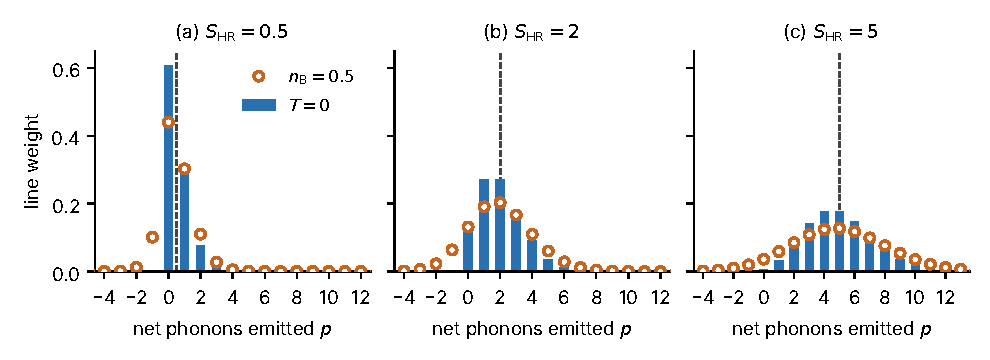
\includegraphics[width=\linewidth]{figures/ch05/fig5_5.pdf}
  \caption{Franck--Condon progressions of a displaced oscillator, for Huang--Rhys factors $S_{\mathrm{HR}} = 0.5$, 2 and 5. Each panel shows the weights of the absorption lines at $E_{\mathrm{ZPL}} + p\,\omega_0$ against the net number $p$ of phonons emitted, for one mode of frequency $\omega_0$ that is the same in both electronic states, in the Condon approximation (dipole independent of the nuclear coordinate). Bars: zero temperature, Poisson weights $\ee^{-S_{\mathrm{HR}}}S_{\mathrm{HR}}^p/p!$; the bar at $p = 0$ is the zero-phonon line. Open circles: mean occupation $n_{\mathrm{B}}(\omega_0) = 0.5$, that is $T = 0.91\,\omega_0$, from the Bessel-function weights of \cref{eq:5.6-bessel}; the lines at $p < 0$ are anti-Stokes lines, which start from thermally excited vibrational states. Dashed line: the mean $p = S_{\mathrm{HR}}$, the same at both temperatures. The zero-phonon fractions at $T = 0$ are 0.61, 0.14 and 0.007.}
  \label{fig:5-fc}
\end{figure}

At finite temperature the initial vibrational state is thermal, and the overlaps $|\langle m_{\mathrm{e}}|n_{\mathrm{g}}\rangle|^2$ for $n > 0$ are needed as well. Summing them with Gibbs weights is a job for the generating function. The absorption line shape is
\begin{equation*}
  \begin{aligned}
  A(E) &= \sum_np_n\sum_m|\langle m_{\mathrm{e}}|n_{\mathrm{g}}\rangle|^2\,\delta\bigl(E - E_{\mathrm{ZPL}} - (m - n)\,\omega_0\bigr) \\
  &= \int_{-\infty}^{\infty}\frac{\dd t}{2\pi}\;\ee^{\ii(E - E_{\mathrm{ZPL}})t}\,\bigl\langle\ee^{\ii H_{\mathrm{g}}t}\op{D}\,\ee^{-\ii H_{\mathrm{g}}t}\op{D}^\dagger\bigr\rangle ,
  \end{aligned}
\end{equation*}
where $p_n$ are the Gibbs weights of the ground-state oscillator (\cref{sec:2.5}). The second form writes each $\delta$-function as the time integral of $\ee^{\ii(E - E_{\mathrm{ZPL}} - m\omega_0 + n\omega_0)t}$, uses $\langle m_{\mathrm{e}}|n_{\mathrm{g}}\rangle = \langle m|\op{D}^\dagger|n\rangle$, and lets $\ee^{\pm\ii H_{\mathrm{g}}t}$ supply the phases $\ee^{\ii n\omega_0t}$ and $\ee^{-\ii m\omega_0t}$; the sum over $m$ is then a completeness sum. The operator $\ee^{\ii H_{\mathrm{g}}t}\op{D}\ee^{-\ii H_{\mathrm{g}}t}$ is $\op{D}$ with $d \to d\,\ee^{-\ii\omega_0t}$, so both exponents are linear in $d$ and $d^\dagger$, and \cref{eq:C.6-product} applies, with $\op{A} = \alpha_{\mathrm{d}}(d^\dagger\ee^{\ii\omega_0t} - d\,\ee^{-\ii\omega_0t})$ and $\op{B} = -\alpha_{\mathrm{d}}(d^\dagger - d)$. The averages are $\langle\op{A}^2\rangle = \langle\op{B}^2\rangle = -S_{\mathrm{HR}}(2n_{\mathrm{B}} + 1)$ and $\langle\op{A}\op{B}\rangle = S_{\mathrm{HR}}[(n_{\mathrm{B}} + 1)\ee^{-\ii\omega_0t} + n_{\mathrm{B}}\ee^{\ii\omega_0t}]$, with $n_{\mathrm{B}} = n_{\mathrm{B}}(\omega_0)$, so that
\begin{equation}
  \bigl\langle\ee^{\ii H_{\mathrm{g}}t}\op{D}\,\ee^{-\ii H_{\mathrm{g}}t}\op{D}^\dagger\bigr\rangle
  = \ee^{-S_{\mathrm{HR}}(2n_{\mathrm{B}} + 1)}\,\exp\Bigl\{S_{\mathrm{HR}}\bigl[(n_{\mathrm{B}} + 1)\,\ee^{-\ii\omega_0t} + n_{\mathrm{B}}\,\ee^{\ii\omega_0t}\bigr]\Bigr\} .
  \label{eq:5.6-Gt}
\end{equation}
It has the form of the generating formula \cref{eq:5.6-gen} for a crystal with a single mode: $2W_\kappa$ becomes $S_{\mathrm{HR}}(2n_{\mathrm{B}} + 1)$, and $\vect{q}\cdot\mathcal{C}_{\kappa\kappa}(t)\cdot\vect{q}$ becomes the second exponent. A kick of momentum $q$ to a single oscillator is the displacement $\op{D}(\ii q\ell_0)$ (\cref{app:C.6}), and it leads to the same expression with $S_{\mathrm{HR}} \to E_R/\omega_0$. The second exponential expands with the generating function of the modified Bessel functions, $\ee^{(z/2)(s + 1/s)} = \sum_ps^pI_p(z)$, taken at $s = [(n_{\mathrm{B}} + 1)/n_{\mathrm{B}}]^{1/2}\ee^{-\ii\omega_0t}$. The coefficient of $\ee^{-\ii p\omega_0t}$ is the weight of the line at $E_{\mathrm{ZPL}} + p\,\omega_0$, for every integer $p$:
\begin{equation}
  w_p = \ee^{-S_{\mathrm{HR}}(2n_{\mathrm{B}} + 1)}\Bigl(\frac{n_{\mathrm{B}} + 1}{n_{\mathrm{B}}}\Bigr)^{p/2}I_p\bigl(2S_{\mathrm{HR}}\sqrt{n_{\mathrm{B}}(n_{\mathrm{B}} + 1)}\bigr) .
  \label{eq:5.6-bessel}
\end{equation}
At $T = 0$ only $p \ge 0$ survives, and $w_p$ returns to the Poisson weights of \cref{eq:5.6-FC}. At $T > 0$ the lines with $p < 0$ appear, and since $I_{-p} = I_p$, $w_{-p}/w_p = \ee^{-p\beta\omega_0}$, detailed balance between the Stokes and anti-Stokes sides. The mean of $p$ is $S_{\mathrm{HR}}$ at every temperature, the slope of \cref{eq:5.6-Gt} at $t = 0$, as the mean recoil energy was in \cref{eq:5.6-sum}.

A real center couples to many modes $k$, each with its own factor $S_k = \omega_k\Delta Q_k^2/2$, and the generating function is the product of factors \cref{eq:5.6-Gt}, one per mode. The total $S_{\mathrm{HR}} = \sum_kS_k$ is the mean number of phonons emitted, and at $T = 0$ the zero-phonon weight is $\ee^{-S_{\mathrm{HR}}}$. With a continuum of modes, the replicas merge into a continuous sideband with the shape of the convolutions of \cref{eq:5.6-multi}, while the zero-phonon line stays sharp, since it involves no phonon. Huang and Rhys derived this structure for the F center of alkali halides, where $S_{\mathrm{HR}}$ is large and the band is broad~\cite{huang1950theory}. \Cref{sec:7.4} applies it to the color centers of silicon and diamond, with their measured Huang--Rhys factors.

\begin{workedexample}{A displaced oscillator}\label{we:5-displaced}
As a toy model we take the bond coordinate of silicon from \cref{sec:5.1}, an oscillator of frequency $\omega_0 = \SI{64.1}{meV}$ whose zero-point length is $\ell_0 = \ell_{\mathrm{zp}} = \SI{0.048}{\angstrom}$ (with the reduced mass $M/2$ of the pair of nuclei, $\ell_0 = (2\cdot\tfrac{M}{2}\cdot\omega_0)^{-1/2}$ is the $\ell_{\mathrm{zp}}$ of \cref{fig:5-scales}). Suppose a localized electronic excitation lengthens the equilibrium bond by $\Delta x$.

\emph{The size of the shift.} A Huang--Rhys factor of two needs $\Delta x = 2\ell_0\sqrt{S_{\mathrm{HR}}} = \SI{0.136}{\angstrom}$, \SI{5.8}{\percent} of the bond length $\sqrt3a/4 = \SI{2.35}{\angstrom}$. A shift of a few times the zero-point length is enough to make the zero-phonon line a minority: the relaxation energy is $S_{\mathrm{HR}}\omega_0 = \SI{128}{meV}$, and the Stokes shift between the means of absorption and emission is \SI{256}{meV}.

\emph{The overlap directly.} The ground-state wavefunction is $\psi_0(x) = (2\pi\ell_0^2)^{-1/4}\ee^{-x^2/4\ell_0^2}$, and the overlap with the same Gaussian centered at $\Delta x$ is
\begin{equation*}
  \langle0_{\mathrm{e}}|0_{\mathrm{g}}\rangle = \frac{1}{\sqrt{2\pi}\,\ell_0}\int\dd x\;\ee^{-[x^2 + (x - \Delta x)^2]/4\ell_0^2}
  = \frac{\ee^{-\Delta x^2/4\ell_0^2}}{\sqrt{2\pi}\,\ell_0}\int\dd x\;\ee^{-x^2/2\ell_0^2 + x\Delta x/2\ell_0^2}
  = \ee^{-\Delta x^2/8\ell_0^2} ,
\end{equation*}
by \cref{eq:C.6-gauss} with $\mu = 1/2\ell_0^2$ and $\eta = \Delta x/2\ell_0^2$, which contributes $\sqrt{2\pi}\,\ell_0\,\ee^{\Delta x^2/8\ell_0^2}$. The squared overlap is $\ee^{-\Delta x^2/4\ell_0^2} = \ee^{-S_{\mathrm{HR}}}$, the zero-phonon weight of \cref{eq:5.6-FC}. For the first replica, $\psi_1(x) = (x/\ell_0)\psi_0(x)$, and the same integral with an extra factor $(x - \Delta x)/\ell_0$ gives $|\langle1_{\mathrm{e}}|0_{\mathrm{g}}\rangle|^2 = S_{\mathrm{HR}}\ee^{-S_{\mathrm{HR}}}$.

\emph{The progression.} For $S_{\mathrm{HR}} = 2$ the weights of the lines with $p = 0$ to 5 phonons are $0.135$, $0.271$, $0.271$, $0.180$, $0.090$ and $0.036$, the middle panel of \cref{fig:5-fc}. The zero-phonon line carries \SI{14}{\percent} of the absorption, and the strongest replicas are those with one and two phonons, which for an integer $S_{\mathrm{HR}}$ are equal.

\emph{Room temperature.} At \SI{300}{K}, $n_{\mathrm{B}}(\omega_0) = 0.091$, the value of \cref{sec:5.3} for the optical phonon. By \cref{eq:5.6-bessel}, the first anti-Stokes line, at $E_{\mathrm{ZPL}} - \omega_0$, has weight $0.021$, and the first Stokes replica $0.249$; their ratio is $\ee^{-\beta\omega_0} = 0.084$. The thermal population thus adds a weak line on the low-energy side of the zero-phonon line, while the mean of the spectrum stays at $E_{\mathrm{ZPL}} + 2\omega_0$.
\end{workedexample}
